
% \section{The effect of network size on weighting errors between spiking neurons}
% - Explanation of Experiment
% - Graph
% - Summary of Graph

\chapter{Results, Analysis and Evaluation}

\section{Testing The Simulation}

Simulation testing was performed experimentally, where observed results were
compared to expected results for any given piece of simulation functionality. In
a project with a larger dedicated pool of resources, 
a more robust testing strategy could have involved co-simulating, where the
network simulation is run alongside a mathematical abstraction that holds
assertions on states in the network and alerts the user when those assertions
are broken.

\subsection{Example of a simple spiking network}
As seen in the first example topology in the previous chapter, figure
\ref{fig:top1}, the simplest arrangement of neurons is a single synapse with a
pre and post synaptic neuron. The membrane potentials of the simulation of such
an arrangement can be seen in figure \ref{fig:PRERES1}
\begin{figure}[h!]
    \centering
    % \addtolength{\leftskip} {-4cm}
    % \addtolength{\rightskip}{-4cm}
    % 
\includegraphics[width=0.06\linewidth]{figures/tops/topexamrestwo.png}\vspace{-3ex}
    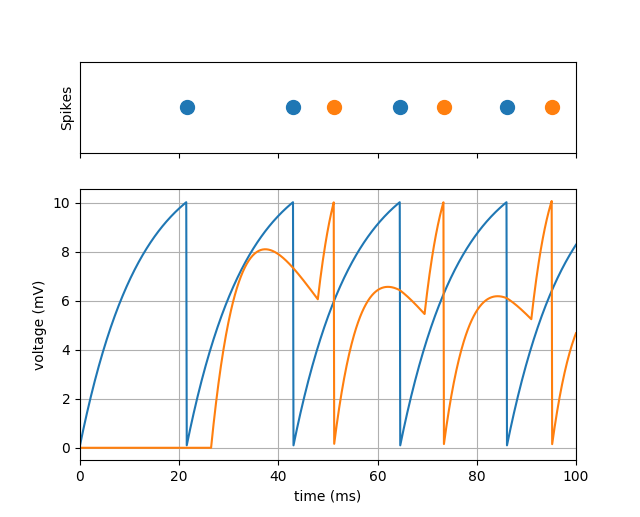
\includegraphics[width=0.7\linewidth]{figures/graphs/DelayBugFixed.png}
    \caption[A simple two-neuron network]{A simple two-neuron network. The input neuron (blue) fires under a constant input current. The second neuron (orange) is synaptically linked, and the synapse has a arbitrary delay of 5ms.}
    \label{fig:PRERES1}
\end{figure}
\subsection{The effect of Gaussian error on weights between spiking neurons}
\begin{figure}[h!]
    \centering
    \addtolength{\leftskip} {-4cm}
    \addtolength{\rightskip}{-4cm}
    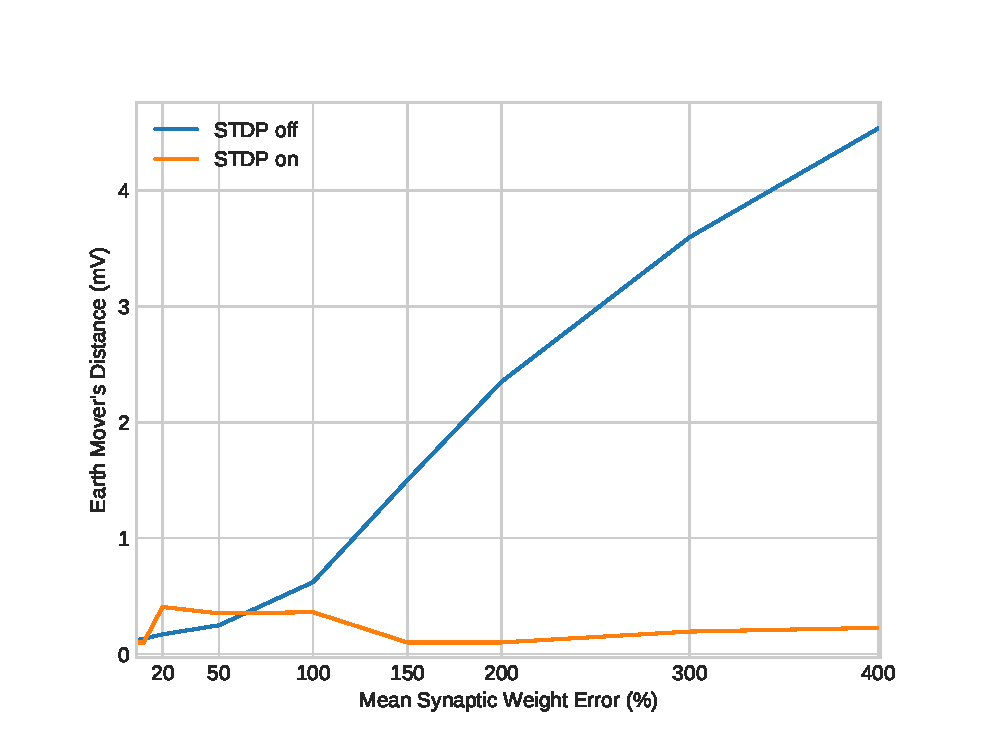
\includegraphics[width=0.7\linewidth]{figures/graphs/RESULT1.eps}
    \caption[Workflow of project simulation]{A schematic that describes the intended workflow for preforming experiments with the simulation tooling that this chapter describes. Cloned simulations can be modified and continue to run in the same manner as their ancestor simulation.}
    \label{fig:RES1}
\end{figure}
- Explanation of Experiment 1
- Graph
- Summary of Graph
\FloatBarrier
\subsection{The effect of STDP on weighting errors between spiking neurons}
\begin{figure}[h!]
    \centering
    \addtolength{\leftskip} {-4cm}
    \addtolength{\rightskip}{-4cm}
    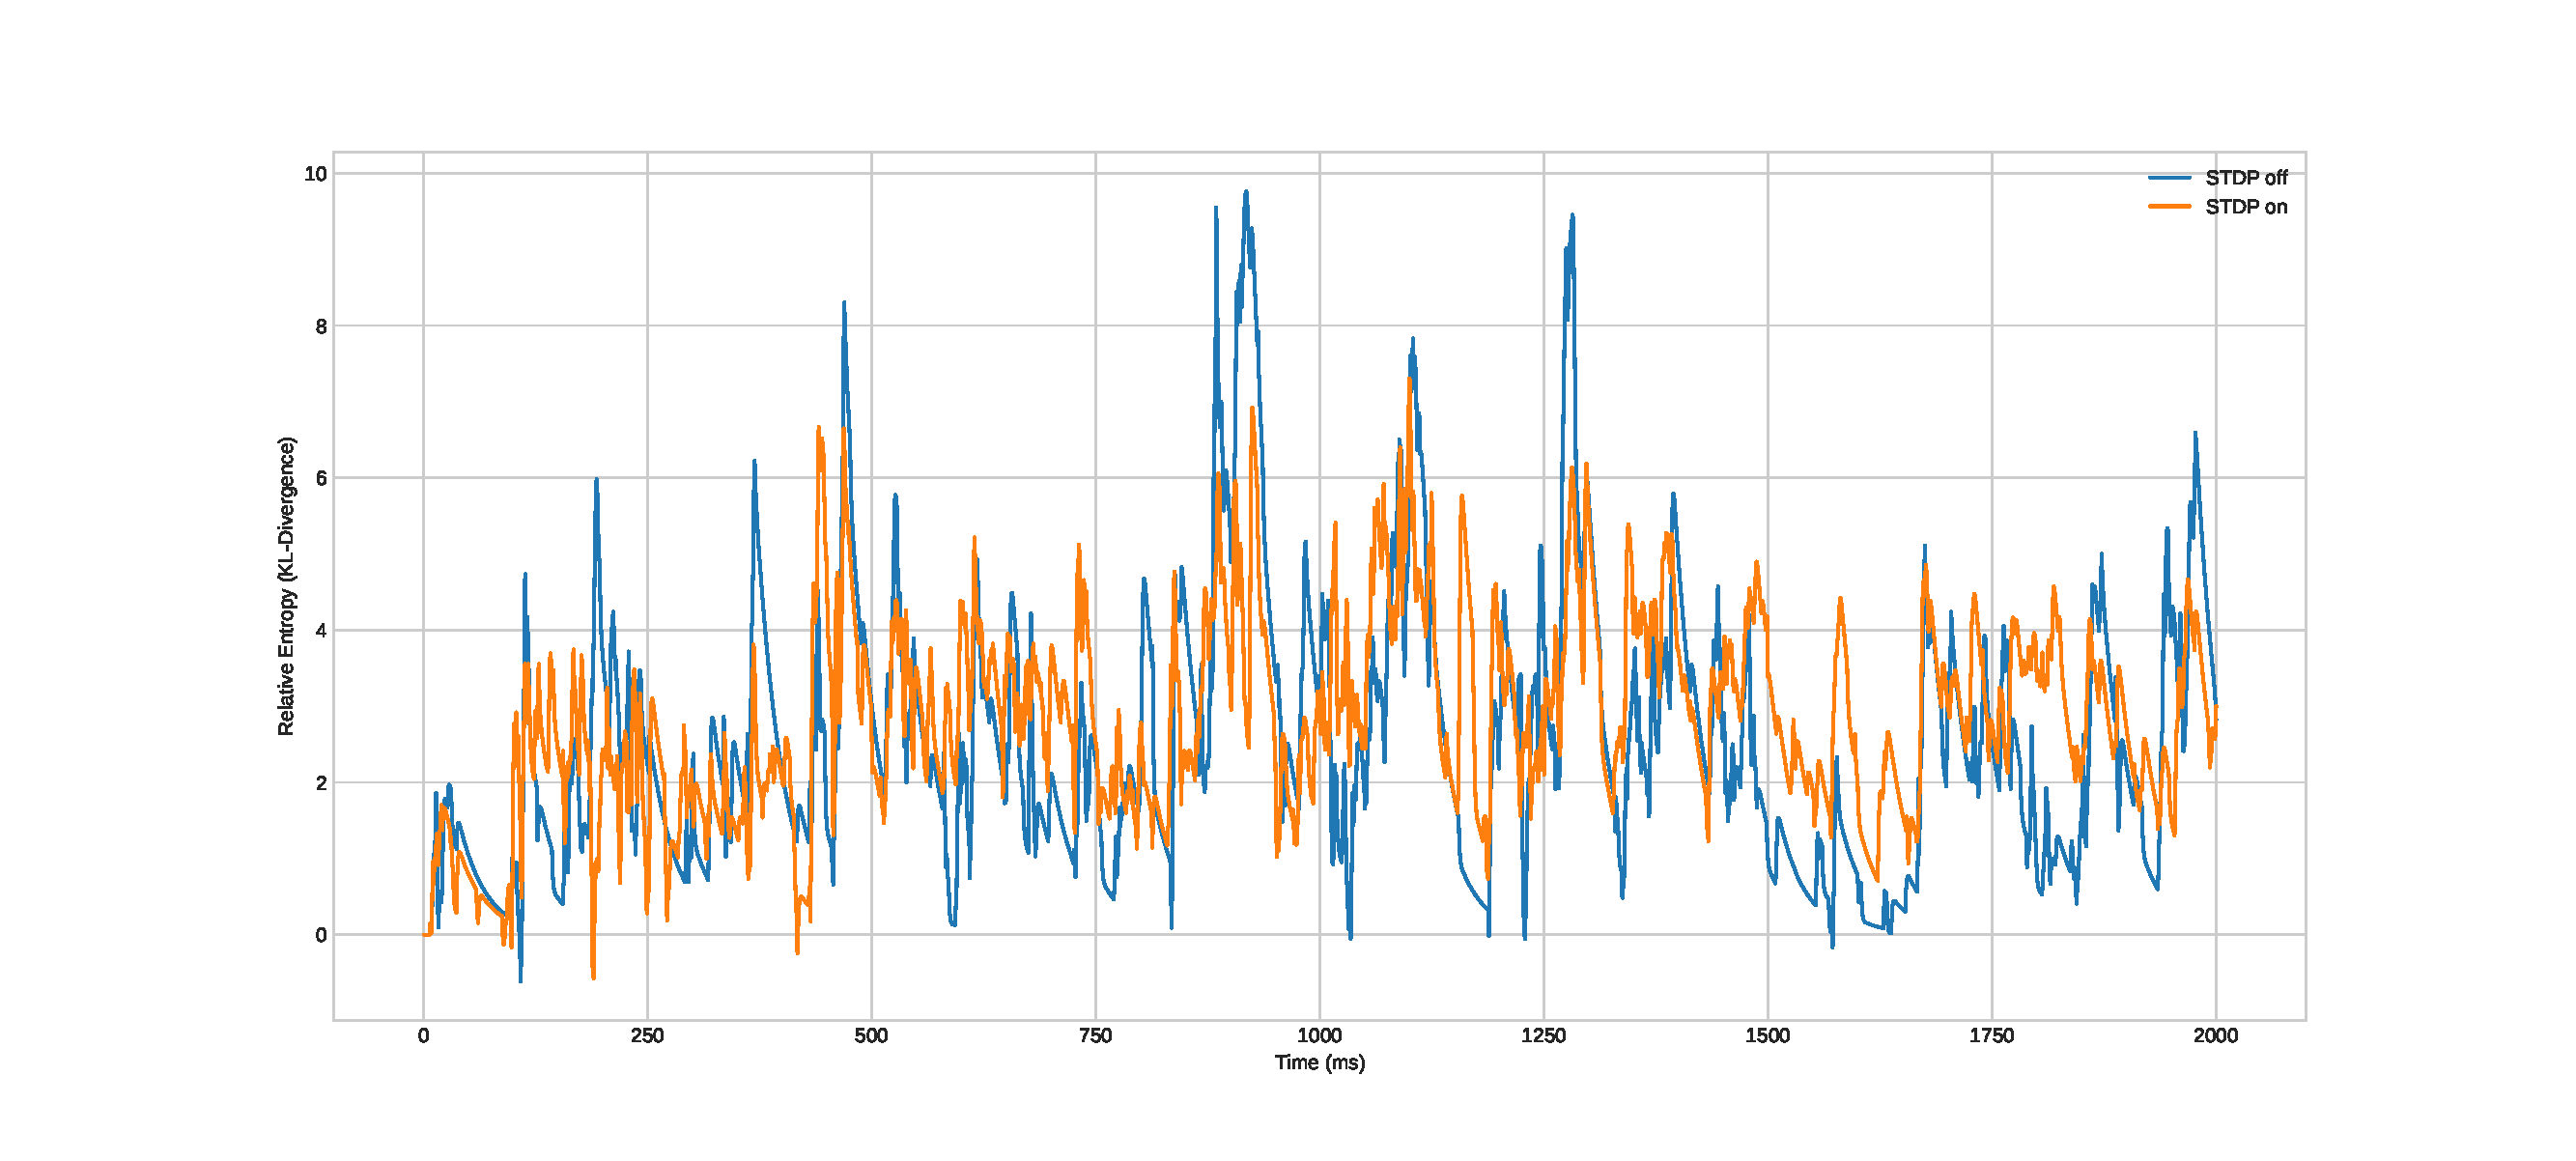
\includegraphics[width=1.6\linewidth]{figures/graphs/RESULT2.eps}
    \caption[Workflow of project simulation]{A schematic that describes the intended workflow for preforming experiments with the simulation tooling that this chapter describes. Cloned simulations can be modified and continue to run in the same manner as their ancestor simulation.}
    \label{fig:RES2}
\end{figure}
- Explanation of Experiment2
- Graph
- Summary of Graph
\FloatBarrier

\section{Result evaluation}

\section{Are they successful? Are they expected?}

- Would have been good to investigate the effect of inhibitory synapses.

- When calculating the difference between spiking distributions, the area under the curve, the total accumulated potential, should have been the same to ensure the results were comparable with both Kullback-Leibler and Earth Movers Distance. Due to the nature of the spiking pattern of the neurons, this was not possible to guarantee, and instead error bars were shown where appropriate. However it would have been preferable, time allowing, to collect multiple results with the same network sizes and mean weighting error, to calculate mean simulation error.

\section{Reflection on development methodology}

- Reactive approach, the requirements of the software adapting as the results
of experiments take shape.

- This is substantially different my original plan of identifying hard
requirements of the system and implementing.
 requirements of the system and implementing. 
requirements of the system and implementing.

- It's much easier to let loose requirements set the direction of travel and
let experiments along the way determine the end result of the software.

- This is partially due to an initial lack of knowledge around the problem
domain. As I understood more about computational neuroscience, domains that
seemed simple took on additional complexity, while previously intractable
concepts became apparent.

- Another benefit of taking an experimental and incremental approach to the
development of the project is that tasks naturally break down into small and
meaningful chunks; each new piece of code does the correct amount of work to
solve a set purpose.

- The caveat to this approach is that it does not lend itself to a holistic
system design or consistent architecture. When defining and writing new
data experiments, the flexibility of decoupled components is ideal, but new code
tends to be purpose built and highly coupled. This would sometimes mean
re-writing code several times as previously finished code had new requirements.

- In general, Conclusions, I’ve found that getting development methodology
“right” is both hard and sort of a misnomer. It depends on the product, the
team, their locations and the workload: what “right” means will change as your
product changes and you move from an experimental development cycle to one with
well formed requirements. One solid way of working throughout a project will
cause friction later down the line.

A lot of time an effort both inside and out of the software development industry
is spent defining `Agile ways of working' \autocite{spolsky_you_2006}, however, from my experiences on this
project, it is better to be flexible and reject workflow rigidity.

Flexibility in ways of working does have its drawbacks however; deadlines must
be set and adhered to throughout a project lest one finds themselves overworked
and unable to produce outcomes that matter externally. In this aspect, my
project would have benefited greatly from a larger sense of responsibility to
myself and the targets I set myself at the beginning of the year. By way of
example, I had originally planned that certain stages of my project could
overrun safely, while others must be completed on time. Sticking to this plan
was far harder than I originally anticipated, and in hindsight it would have been
wise to re-scope the project as soon as it was clearly the best course of action,
instead of carrying a metaphorical weight that it was clear couldn't reach the
finish line.


\section{Ethical considerations for brain simulation}


In "Taking superintelligence seriously: Superintelligence: Paths, dangers,
strategies", Nick Bostrom argues that \ldots
\autocite{bostrom_superintelligence_2014}

\subsection{Pain and suffering in brain simulation}

\autocite{faggella_preventing_2019}
\autocite{singler_existential_2019}
 
\subsection{The rights of a simulation}

\subsection{Kinder artificial intelligence}
probably could go in conclusion. Cite lesswrong dude.
% https://wiki.lesswrong.com/wiki/Friendly_artificial_intelligence

% Is a brain simulation alive? 
% If accurate enough, how separable is a human and a brain simulation from that human?
% Is it ethical to allow a brain simulation to feel pain? 